\section{A modern re-implementation}

There are three main forms in which Signum documents still exist today: printed, stored in the original file format or exported as plain text \cite{xchem2001atari}.

In print, the text is readable but any possibility of editing the document in the future is lost. In the original format, no information is lost but using it requires running the original software, which is only available for a discontinued operating system. In plain text, the character order is preserved, but graphical features like images, formulas or foreign language fonts are lost.

The apparent solution is to take the original format, which has all relevant information still intact, and convert it into a format that can be used with modern tools.

Thus, based on the knowledge I derived from experiments with running Signum! in an emulator (cf. \autoref{sec:emulator}), the few pieces of code working with these file formats that I found on the internet and reading the \textit{Das Signum! Buch} \cite{ritzhaupt1988signum}, I implemented a software that is able to read, process and convert Signum!2 documents.

This software is available for others to use and is implemented using the Rust programming language \cite{xipho2020sdotool}.

\subsection{Using the Rust programming language}

Rust is a systems programming language that presents itself with the tagline \textit{A language empowering everyone to build reliable and efficient software}\footnote{\url{https://rust-lang.org}}. It comes with a package manager called \textit{Cargo} and built-in capabilities for dependency management, automatic tests, generating documentation from code and comments and a large standard library of utilities.

Initially developed as a hobby project, it was adopted as a research project by \textit{Mozilla} in 2010 and released to a wider audience in 2015. Starting out from the position to \textquote{Concentrate on known ways of achieving more safety, more concurrency, less mess} \cites{rustNothingNew, rustRefInfluences}, it has since been adopted at all of the big 5 tech companies (Google, Apple, Facebook, Amazon, Microsoft) and has recently established its own foundation \cite{mzla2021rustfoundation}.

Using Rust, I could build on top of existing libraries, such as \textit{nom} for parsing file formats and \textit{image} for encoding images to modern formats, just by adding their name to a list of dependencies \cites{geal2020nom, rs2020image}. In the same spirit, I have released reusable components of my work to that same package registry \cites{xipho2021signum, xipho2020pdfc, xipho2020ccitt}.

Rust is also useful in this case, because the language makes it easy to write correct code by modeling edge cases in data types. There is no special \texttt{null} value that indicates the absence of a value. If a value of type \texttt{T} may not be available, then the type of that value is \texttt{Option<T>} and, which must be \textit{unwrapped} before accessing the inner value. A program always halts with a useful error message by default if a problem is encountered.

Finally, it's normal for errors to occur in the case of reverse engineering a file format. Using a languages that provides a reasonable certainty that the code does what is intended, if it compiles successfully, implies that the error is most likely caused by a misunderstanding of the file format and not by a mistake in the implementation.

\subsection{PostScript / PDF}

Ever since the ATARI and Signum! were discontinued, users of the software
were interested in exporting their documents for use in other systems. While there are recommendations on how to do just that, all of them have their own limitations.

Commonly, the request was to be able to open Signum! files with other word processing programs like \textit{StarOffice} or \textit{MS Word}. In this section, I'll explain why I focused my attention on PDF as an output format instead.

\subsubsection{Conversion to modern formats}

Today, the Signum! file format is no longer in use. The only software that could read it was only available on the the ATARI ST. There was a conversion software (\textbf{TEXTCONV.PRG}) packaged with another word processor for the ATARI called \textit{Papyrus}, which could export to \acrfull{rtf}. However, the result isn't great for anything that isn't plain text.

Signum! itself had the ability to export to ASCII, which also lacked all of the advanced formatting options. The next version, Signum!3 could also read the files from the previous version but it comes with its own custom file format that no other programs support.

The third strategy was to use a virtual printer to print Signum! documents to a set of images instead of paper on a real printer. This had the advantage of preserving the documents at a very high quality and accuracy. The downside is that, even with subsequent processing using \textit{Optical Character Recognition}, it's prone to errors and hard to search or re-use the text.

\subsubsection{A page definition language}

As explained in \autoref{sec:sdoc_tebu}, Signum documents store their text based on the position of the characters, not their order in the text. An expression like $Q_2$ would be typeset as a $Q$ on one line and a small $2$ on a line further down. To turn this into a tag based document language like \acrshort{html} or \textit{MS Word 2007 (docx)} requires interpreting these relationships.

Ideally, these positions could just be re-used in the new format. The relevant goal is keeping information about the characters so that the text is searchable. The text alone does not have contain information to produce an accurate copy of the original. This is exactly what a \acrfull{pdl} is used for.

\textit{PostScript} is a programming language crated by \textit{Adobe} and is most commonly used as a \acrlong{pdl}. It provides built-in commands like \texttt{moveto} and \texttt{setfont} that manipulate a graphics model that is ultimately sent to an output device with the \texttt{showpage} command.

\textit{\acrshort{pdf}} is a file format also created by \textit{Adobe} that is based on PostScript. The main difference is that PDF is a structured container format that mandates pages and fonts to be specified in a certain way at a pre-defined location, it only provides a subset of all PostScript commands and uses shorter names for them.

So, to translate a \Signum{} file, the approach I chose was to place every character in the correct position independent of all other characters and to gradually introduce logic that removes unnecessary commands. Examples for the latter would be zero-length moves between adjacent characters or switching to the font that's currently active.

\subsection{Bitmap Fonts}

Another challenge in recreating Signum! documents in modern formats were the fonts. As mentioned earlier, it used a set of custom file formats that contained the glyphs for each character in a charset depending on the output device.

Fonts are typically crated as \textit{outlines} by a company called a \textit{font foundry}. These outlines are then \textit{rasterized} at different sizes, that is converted into a format that specifies which positions on a paper or display should be coloured.

One description of this process for a commercial typewriter of the 1980s can be found in a memo by employees of \textit{Bell Labs} \cite[Page 7]{bwk1980summer}, which was the research \& development department of US-American telephone company AT\&T well-known for the development of the UNIX operating system.

These intermediary file formats are called \textit{bitmap fonts} and contain little pixel images for every character or ligature in the font. Both the ATARI ST and the X11 window system first released in 1984 used bitmap fonts initially \cite{tosVDIfontHdr} \cite{ffPCFFormat}.

\begin{figure}
    \centering
    \fbox{\begin{varwidth}{\textwidth}
    $\bs\bs\bs\bs\bs\bs\bs\bs\bs\bs\bs\bs\bs\bs\bs\bs\bs\bs\bs$\\[-1mm]%
    $\bs\bs\bs\bs\bs\bs\bs\bs\bs\bs\bs\bs\bs\bs\bs\bs\bs\bs\bs$\\[-1mm]%
    $\ws\ws\ws\bs\bs\bs\bs\bs\bs\ws\ws\ws\ws\ws\ws\ws\bs\bs\bs$\\[-1mm]%
    $\ws\ws\ws\bs\bs\bs\bs\bs\bs\ws\ws\ws\ws\ws\ws\ws\bs\bs\bs$\\[-1mm]%
    $\ws\ws\ws\bs\bs\bs\bs\bs\bs\ws\ws\ws\ws\ws\ws\ws\bs\bs\bs$\\[-1mm]%
    $\ws\ws\ws\bs\bs\bs\bs\bs\bs\ws\ws\ws\ws\ws\ws\ws\bs\bs\bs$\\[-1mm]%
    $\ws\ws\ws\bs\bs\bs\bs\bs\bs\ws\ws\ws\ws\ws\ws\ws\ws\ws\ws$\\[-1mm]%
    $\ws\ws\ws\bs\bs\bs\bs\bs\bs\ws\ws\ws\ws\bs\bs\bs\ws\ws\ws$\\[-1mm]%
    $\ws\ws\ws\bs\bs\bs\bs\bs\bs\ws\ws\ws\ws\bs\bs\bs\ws\ws\ws$\\[-1mm]%
    $\ws\ws\ws\bs\bs\bs\bs\bs\bs\ws\ws\ws\ws\bs\bs\bs\ws\ws\ws$\\[-1mm]%
    $\ws\ws\ws\bs\bs\bs\bs\bs\bs\bs\bs\bs\bs\bs\bs\bs\ws\ws\ws$\\[-1mm]%
    $\ws\ws\ws\bs\bs\bs\bs\bs\bs\bs\bs\bs\bs\bs\bs\bs\ws\ws\ws$\\[-1mm]%
    $\ws\ws\ws\bs\bs\bs\bs\bs\bs\ws\ws\ws\ws\bs\bs\bs\ws\ws\ws$\\[-1mm]%
    $\ws\ws\ws\bs\bs\bs\bs\bs\bs\ws\ws\ws\ws\bs\bs\bs\ws\ws\ws$\\[-1mm]%
    $\ws\ws\ws\bs\bs\bs\bs\bs\bs\ws\ws\ws\ws\bs\bs\bs\ws\ws\ws$\\[-1mm]%
    $\ws\ws\ws\bs\bs\bs\bs\bs\bs\ws\ws\ws\ws\ws\ws\ws\ws\ws\ws$\\[-1mm]%
    $\ws\ws\ws\bs\bs\bs\bs\bs\bs\ws\ws\ws\ws\ws\ws\ws\ws\bs\bs$\\[-1mm]%
    $\ws\ws\ws\bs\bs\bs\bs\bs\bs\ws\ws\ws\ws\ws\ws\ws\ws\bs\bs$\\[-1mm]%
    $\ws\ws\ws\bs\bs\bs\bs\bs\bs\ws\ws\ws\ws\ws\ws\ws\ws\bs\bs$\\[-1mm]%
    $\ws\ws\ws\bs\bs\bs\bs\bs\bs\ws\ws\ws\ws\ws\ws\ws\ws\bs\bs$\\[-1mm]%
    $\bs\bs\bs\bs\bs\bs\bs\bs\bs\bs\bs\bs\bs\bs\bs\bs\bs\bs\bs$\\[-1mm]%
    $\bs\bs\bs\bs\bs\bs\bs\bs\bs\bs\bs\bs\bs\bs\bs\bs\bs\bs\bs$
    \end{varwidth}}
    \caption{A pixel image for the letter \textbf{\fontfamily{bch} \selectfont E} in the \textit{Bitstream Charter} font in bold at size $24$. \label{fig:bitmap_letter}}
\end{figure}

The first step of my work on \Signum fonts was to figure out the layout of the \textbf{E24}, \textbf{P24} and \textbf{L30} font files and find the pixel images for every character. Fortunately, letters are relatively easy to find when looking at the binary representation of a file. There are usually far fewer alternations between zeroes and ones i.e. black and white in bitmaps that in numeric data.

\subsubsection{TeX + Metafont}

The \TeX{} typesetting system was released in 1986 with the goal of producing documents of \textit{the best} quality. One way that the author, Donald Knuth, intended to achieve this was by creating a program called \textbf{METAFONT} that would take a outline description of the characters of a font and translate them into bitmap fonts of the correct resolution on demand when a \TeX{} document was compiled.

Originally, \TeX{} documents were turned into a format called \textbf{DVI} (\textit{device-independent}) before being sent to a printer. Most modern users of \LaTeX{} use the \texttt{pdflatex} program, which turns \TeX{} files directly into \acrshortpl{pdf}. But it is still possible to use the original toolchain.

The program \texttt{latex} turns a \TeX{} file that uses \LaTeX{} macros (e.g. \texttt{\textbackslash documentclass}) into a \texttt{*.dvi} file. The program \texttt{dvips} turns the DVI file into a \textit{PostScript} program and a PostScript interpreter like \textit{Adobe Distiller} or \textit{GhostScript} turns that program into a PDF file.

It's possible to tell \texttt{dvips} to embed the bitmap fonts generated by METAFONT into the PostScript program. By reverse-engineering how that embedding works, I could substitute the bitmaps that I extracted from the \Signum{} fonts. Ultimately, this is the opposite of what people commonly want\footnote{\url{http://www.texfaq.org/FAQ-pkfix}} and the end result is a standard \textit{Adobe Type3} font.

As with a lot of this project, my first priority was to produce something that produces a recognizable result, then improve my understanding of how it works and eventually replace parts of the system with technologies that are better suited for the task at hand.

\subsubsection{Ghostscript and CCITTFaxDecode}

With the ability to transform \Signum{} texts into PostScript programs, the next step was to compile these programs into PDFs using \textit{Ghostscript} and understanding the way that text and fonts were encoded there.

The fonts were still stored as Adobe Type3 but this time, the individual pixel images for the glyphs were encoded by an algorithm called \textit{\acrshort{ccitt}FaxDecode}. That is the name PDF uses to refer to \textit{International Telecommunications Union (ITU), Recommendations T.4 and T.6} \cites{murray1996ccitt, ccitt1988t4, ccitt1988t6}, originally published in November of 1988.

These algorithms were specifically developed to be good at compressing text documents for use in fax machines. They work particularly well for documents that have a small number of changes between black and white on every line of pixels and which don't change much from one such line to the next.

To be able to use this compression for \Signum{} fonts, I created a \acrshort{ccitt} Group 4 2-Dimensional encoder and a decoder in Rust and made them publicly available\footnote{\url{https://xiphoseer.github.io/sdo-tool/implementation\#ccitt-t4-t6}}.

% (maybe TROFF)
\label{sec:encoding}
\subsection{Font Encoding}

The final challenge related to \Signum{} fonts was to determine which characters were actually provided as part of a charset. A person can look at the bitmap of character number 65 of the \textbf{ANTIKRO} charset and decide that it is the letter \textit{A}, but that involves a lot more work for an automatic system.

Fortunately, the mapping of numbers to keys on the ATARI keyboard is always the same, so all fonts that were just visual variations of these same characters used the same standard mapping\footnote{\href{https://github.com/Xiphoseer/sdo-tool/blob/196fbf9e79c127cb6bfda1a5bb91e51581d050b1/crates/sdo-pdf/src/font.rs\#L20-L44}{Xiphoseer/sdo-tool:/crates/sdo-pdf/src/font.rs\#L20-L44}}. This standard is mostly consistent with the printable characters in the \textit{American Standard Code for Information Interchange (ASCII)}, one of the foundational standards in computing. However, the \Signum{} encoding uses the numbers $1$ to $31$, which are assigned to non-printable control codes in ASCII, for characters typed in using the numpad.

\begin{figure}[h]
    \centering
    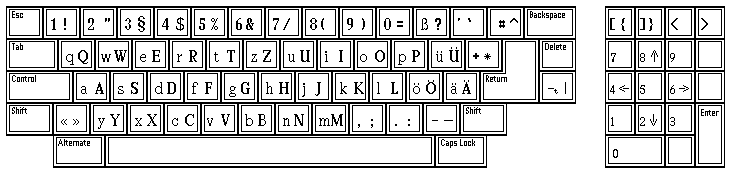
\includegraphics[width=\columnwidth]{img/ANTIKRO.png}
    \caption{The document \textbf{KBANTIK.SDO} that is distributed with \Signum{}. It provides a visual reference to determine which physical key corresponds to which character number, independent of the current character set}
    \label{fig:my_label}
\end{figure}

The computing industry has since created the \gls{Unicode} standard, which aims to assign a single number called a \gls{codepoint} to every character that is used in any amount of significant documents written in a current or historic language\funfact{This occasionally has unintentional side-effects like adopting Emoji worldwide when integrating the japan-specific \textit{ShiftJIS} encoding\href{https://www.theverge.com/2013/3/4/3966140/how-emoji-conquered-the-world}{$[A]$}\href{https://www.youtube.com/watch?v=5OPkGQoPeHk}{$[B]$}}.

This is useful to solve the same kind of challenges that \Signum{} was used for: Writing mixed-language text with built-in support for languages like Greek or Hebrew.

\gls{Unicode} uses \textit{mapping tables} to describe the transformation of one text encoding into \glspl{codepoint} \cite{unicode2015atarist}. As every \Signum{} charset can represent an encoding as well as a font, it's possible to create mapping files for some of the charsets \cite{xipho2020antikro} and re-use them for other character sets which match the same encoding.